\chapter{Modelo GRAND}
\label{cap:grand}

No modelo GRAND são tratados três aspectos do gerenciamento de dados: transferência automática dos dados de entrada para o local onde o arquivo será necessário; o envio de resultados é controlado evitando congestionamento da rede; priorização de localidade no disparo de tarefas para não haver transferências desnecessárias de dados degradando o desempenho. Através de uma hierarquia de gerenciadores (Figura 1) é feito o disparo e controle das aplicações. o \emph{Application Manager} (AP) recebe uma submissão de aplicação através de um usuário, os APs mandam os \emph{Submission Managers} (SM) descrições de tarefas assim, sob demanda, são instanciados os \emph{Task Managers} (TM) para controlar a submissão de tarefas a escalonadores de domínios específicos da grade, esses escalonadores recebem requisições dos TMs fazendo a execução das tarefas propriamente ditas.

Pelo fato de que, na atualidade, ambientes grades envolvem principalmente instituições de ensino em aplicações usualmente classificadas como aplicações científicas, o escopo do GRAND é limitado as seguintes itens. 

\begin{enumerate}
    \item heterogeneidade, lembrando que isto afeta diretamente a política de escalonamento por necessitar de saber as características distintas de hardware e software; 
    \item grande número de submissão de tarefas, referindo-se a aplicações que geram centenas ou milhares de processos; 
    \item ausência de comunicação por troca de mensagens, pelo fato da necessidade de inúmeros aspectos nas fases de agrupamento e mapeamento serem considerados; 
    \item interdependência de tarefas, devido ao compartilhamento de arquivos; 
    \item manipulação de grande número de arquivos pelas tarefas; 
    \item o uso de arquivos grandes, através de técnicas como \emph{staging} e \emph{caching}, minimizando a perda de desempenho em função da latência de transmissão; 
    \item segurança, assume-se que exista uma conexão segura entre os nós da grade; 
    \item descoberta dinâmica de recursos; 
    \item gerenciador de recursos local em cada nó; 
    \item uma tarefa é executada em um RMS até sua finalização;
\end{enumerate}

\section{Característica das Aplicações}

Baseando-se em aplicações típicas para ambientes de grades, comunicando-se via troca de arquivo, conhecimento do número de processo a serem criados e sem troca de mensagens, é proposta a seguinte taxonomia de aplicações \cite{Vargas2003, Vargas2005, Mangan2006}

\begin{itemize}
	\item tarefas independentes \emph{\textbf{independent tasks}} ou seja, as tarefas não possuem dependência entre si. Muitas vezes chamado de \emph{bag-of-tasks}.
	\item tarefas fracamente acopladas \emph{\textbf{loosely-coupled tasks}} tarefas com poucos pontos de compartilhamentos, aplicações dividas em fases ou sequência.
	\item tarefas fortemente acopladas \emph{\textbf{tightly-coupled tasks}} grafos complexos, aplicações em lógica com restrições.
\end{itemize}

\begin{figure}[htb]
\begin{center}
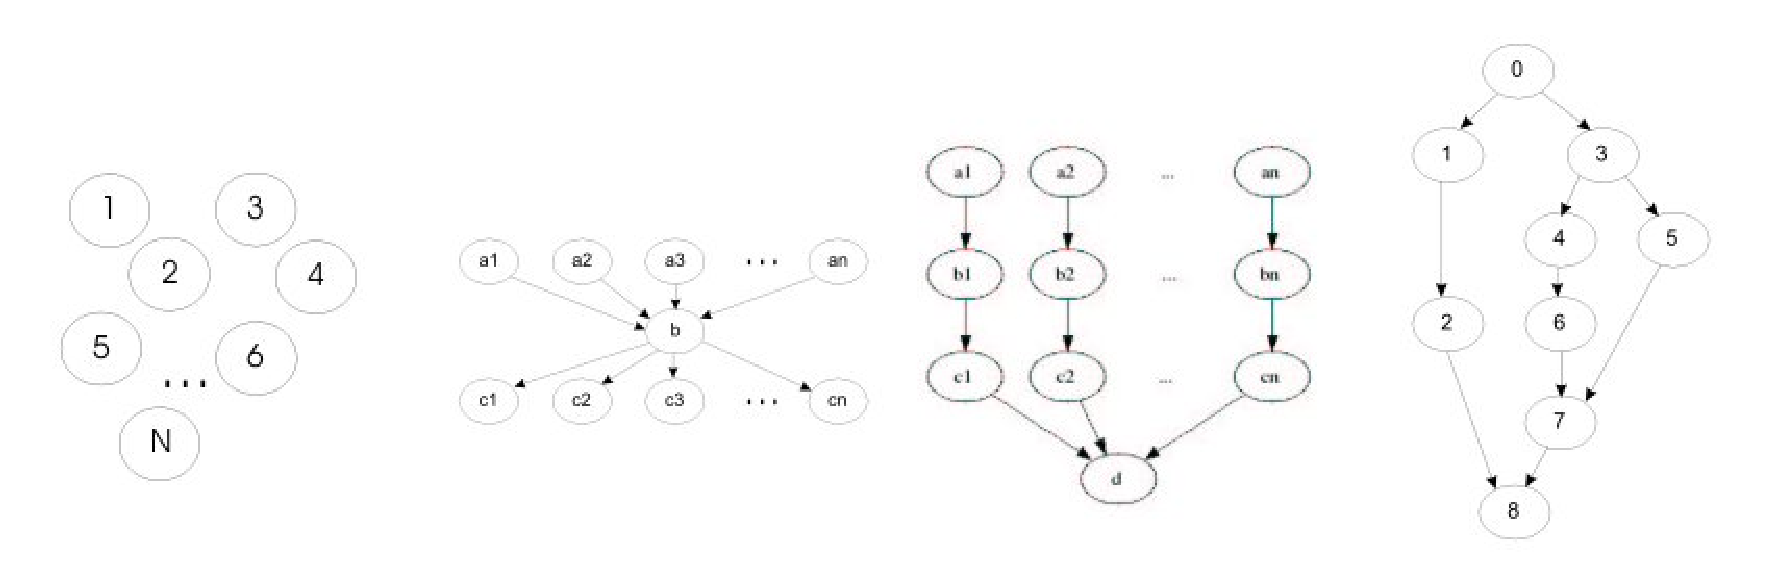
\includegraphics[scale=0.5]{./img/TaxonomiaAplicacoes.eps}
\caption{Categorias de aplicações de grade: (a) \emph{independent tasks}, (b) \emph{loosely-coupled task(phase)}, (c) \emph{loosely-coupled tasks (pipeline)} e (d) \emph{tightly-coupled tasks}}
\label{fig:Taxonomia_Aplicacoes}
\end{center}
\end{figure}

\section{Gerenciamento de Dados}

Ainda há muito o que ser feito nesta questão, até então o tratamento dos dados é resolvido através de soluções distintas. A preocupação principal de vários trabalhos \cite
{GridFTP,LegionFS} é com dados em forma de arquivos.

No GRAND, o gerenciamento de arquivos é apenas com \emph{stage in} e \emph{stage out}, ou seja, enviar os dados para o local de processamento e retorno de resultados. 

A máquina de submissão (\emph{submit machine}) é a máquina que o usuário submete um grande número de tarefas. Nesta máquina exige um gerenciador encarregado de submeter tarefas para outros gerenciadores guardando o resultado final das tarefas sem preocupar-se com os detalhes. Esse gerenciador executa ou utiliza gerenciadores do sistema que fazem o escalonamento preocupando-se em privilegiar o local dos dados. O envio para a máquina (\emph{home}) é controlado para evitar um congestionamento.

A liberação de carga da máquina que foi usada para disparar a aplicação é a principal vantagem deste esquema.


\section{Particionamento}

O problema tratado no contexto pressupõe que as aplicações submetidas são formadas por tarefas passíveis de dependência na ordem de execução, determinadas pelos dados de entrada e saída, não realizando comunicação por troca de mensagem.

Uma aplicação pode ser representada por um grafo direcionado acíclico (DAG - \emph{Directed Acyclic Graph}) onde o vértice representa uma tarefa e as arestas sua ordem de precedência entre outras tarefas. Este DAG é particionado em sub-grafos para que eles possam ser alocados de forma eficiente em diferentes processadores. O algoritmo DSC (\emph{Dominant Sequence Clustering}) de complexidade \emph{O((v+e) log v)} onde \emph{v} é o número de tarefas e \emph{e} o número de arestas.

\section{Modelo de Gerenciamento}

Três aspectos do gerenciamento de dados são tratados no modelo GRAND:

\begin{itemize}
	\item transferência dos dados de entrada automaticamente para o local onde o arquivo é necessário;
	\item envio de resultados de forma controlada, evitando congestionamento, levando em conta o grande volume de dados;
	\item para evitar transferências desnecessárias de dados transientes, o escalonamento prioriza localidade no disparo de tarefas e degradação do desempenho;
\end{itemize}

Uma hierarquia de gerenciadores é usada para o disparo e controle das aplicações conforme ilustrado na figura 3.2.

\begin{itemize}
	\item \textbf{nível 0} aplicação submetida pelo usuário em uma máquina através do \emph{Application Manager}(AP).
	\item \textbf{nível 1} os APs enviam aos \emph{Submission Managers}(SM) descrições de tarefas.
	\item \textbf{nível 2} os \emph{Task Managers}(TK) são instanciados sob demanda pelos SMs com o propósito de controlar a submissão de tarefas para escalonadores de domínios específicos da grade.
	\item \textbf{nível 3} os TKs enviam requisições para os escalonadores a executar de fato as tarefas.
\end{itemize}

\begin{figure}[htb]
\begin{center}
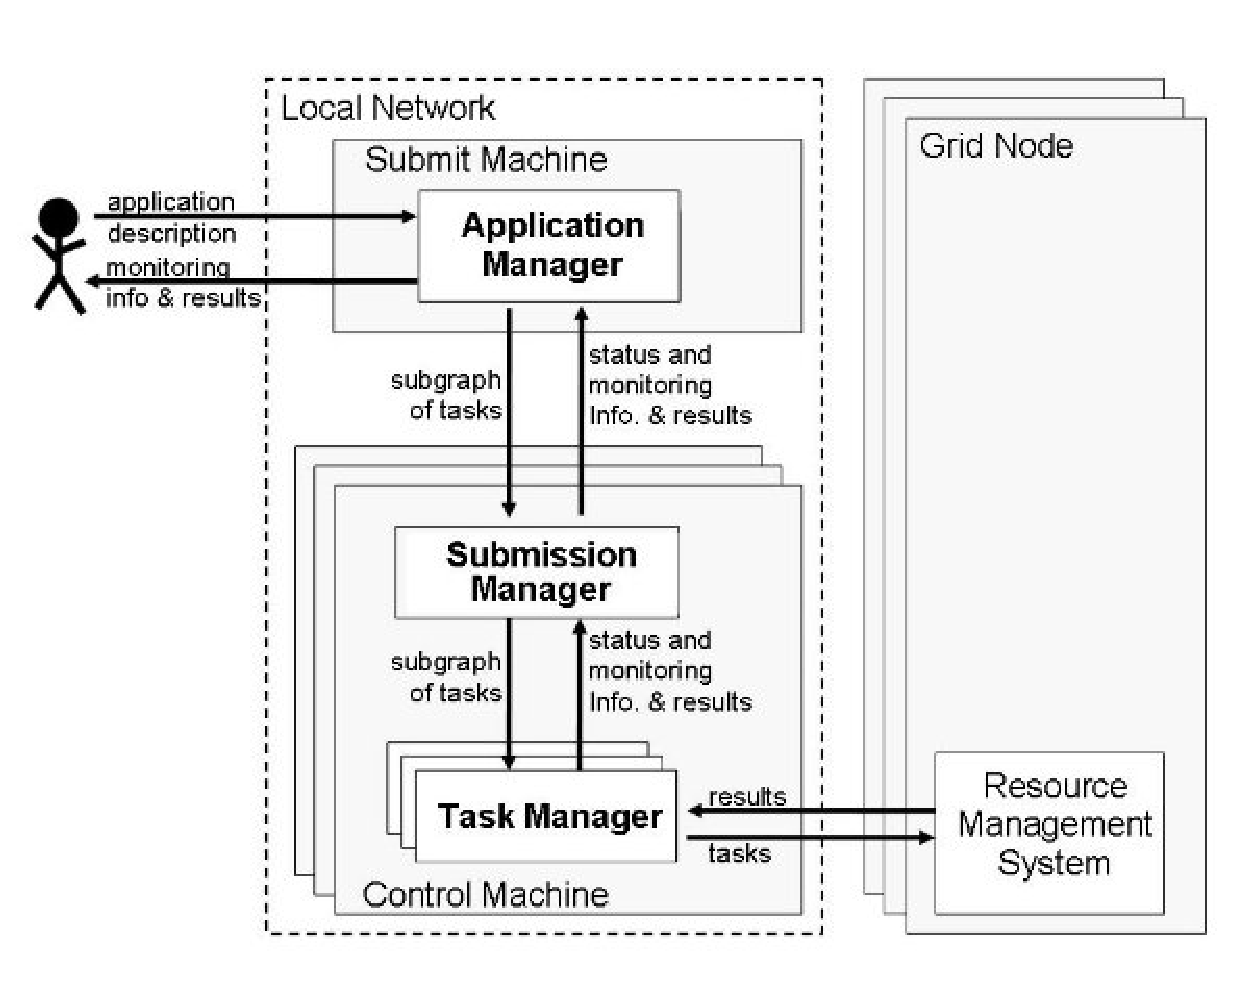
\includegraphics[scale=0.7]{./img/grand.eps}
\caption{Principais componentes do modelo hierárquico de gerenciamento de tarefas}
\label{fig:Modelo_Grand}
\end{center}
\end{figure}

O AP encarrega-se de receber um arquivo de entrada com a descrição da tarefa, particiona as tarefas em sub-grafos para enviá-los para SMs distintos vizando manter a localidade dos dados diminuindo a comunicação entre os SMs e apresenta ao usuário informações do estado da execução da aplicação.

No SM é decidido a localidade dos sub-grafos com base em informações dinâmicas sobre os recursos computacionais, indicação do estado da execução e falhas de comunicação periódicas com o SMs, recuperação de falhas através de um registro persistente (\emph{log}), criação e monitoração dos TKs e verificar a continuação ou não da execução de tarefas em máquinas que forem liberadas ou que houverem falhas.

As responsabilidades dos TKs são comunicar-se com um escalonador de um determinado domínio garantindo a execução remota, garantir a ordem da execução coforme dependência de dados e garantir a disponibilidade dos dados de entrada bem como o recebimento dos dados de saída.

A hierarquia do modelo proposto realiza um balanceamento da carga computacional utilizada para controlar a execução das tarefas, evitando seu sobrecarregamento. Deste modo a perda de dados por congestionamento da rede é evitado. E, também, é permitido que escalonadores já existentes sejam integrados em um único ambiente de escalonamento.

\section{Protótipo AppMan}

O protótipo possui um \emph{Application Manager} que dispara e monitora as aplicações em máquinas de uma rede local e cada máquina possui um \emph{Submission Manager}. Estes SMs não se comunicam nem reconhecem a localização de outros SMs. Assim sendo, as aplicações só funcionam em situações que o particionamento gere grafos totalmente disjuntos, ou seja, sem dependência entre SMs e cada sub-grafo executa até o final sem falhas.

A especificação da aplicação é feito pela linguagem GRID-ADL(\emph{Grid Application Description Language}), onde o usuário descreve apenas características das tarefas incluindo arquivos manipulados. O \emph{parser} para leitura do arquivo de descrição e a inferência do DAG é implementado na ferramenta JavaCC \cite{javacc}. Assim que obtém-se o DAG a execução é iniciada. Na implementação das fases de submissão e controle da execução usou-se a linguagem Java dentro do ambiente EXEHDA (\emph{Execution Environment for High Distributed Application}) \cite{exehda}.

A figura 3.3 é um exemplo de apenas três linhas uma definição de números de tarefas. Neste exemplo é definido um grafo independente com seis tarefas.A aplicação irá executar seis simulações Monte Carlo. Cada uma recebendo um arquivo de entrada diferente.

\begin{figure}[htb]
\begin{center}
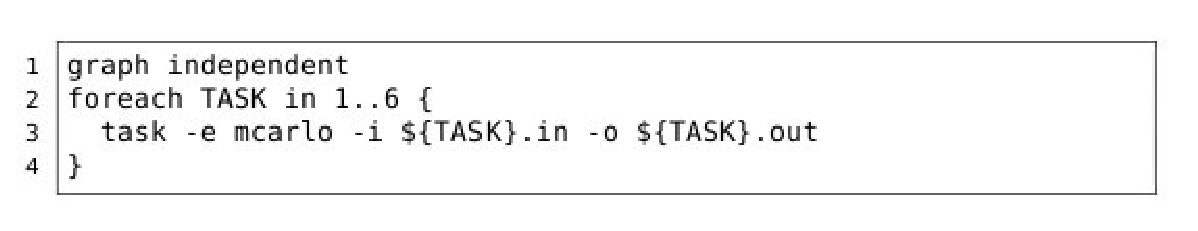
\includegraphics[scale=0.7]{./img/grid-adl.eps}
\caption{Arquivo de entrada para DAG}
\label{fig:Arquivo_DAG}
\end{center}
\end{figure}

EXEHDA é um modelo voltado a aplicações distribuídas, comtemplando mobilidade de hardware e software. As aplicações são baseadas no paradigma de programação do projeto ISAM (Infra-estrutura de Suporte às Aplicações Móveis).

O passo um da figura x representa o usuário submetendo um arquivo de descrição em GRID-ADL. É feito um \emph{parser} no arquivo e o grafo da aplicação é colocado em memória. Um algoritmo de cluster é executado e os sub-grafos são gerados. O AM é inicializado então os AMs instanciam SMs (passo 2), distribuindo alguns sub-grafos para SMs. O arquivo de entrada e o executável são adquiridos pelo \emph{webservice} (passo 3). Um novo SM é instanciado para cada aplicação em cada máquina especificada. Após a criação dos SMs, o AP atribui sub-grafos para cada SM. Os SMs reportam para o AM o progresso das tarefas. Cada SM, independente, verifica a lista de máquinas disponíveis e escolhe onde irá executar, através de um \emph{round-robin} (passo 4).

Um TM é instanciado, o qual cria tarefas remotas e monitora até estarem completas. Antes de inciar a execução de uma tarefa, AppMan transfere todos arquivos de entrada para um diretório temporário na máquina remota onde a tarefa será executada. Cada SM atualiza informação, através do serviço de informação do EXEHDA, do nós disponíveis. 

Alguns mecanismos de tolerância à falhas foram implementados. Na transferência dos arquivos de entrada, não for possível enviar um arquivo, assume-se um falha temporária de comunicaçào e tenta-se novamente a transferência. Se, ao término de uma tarefa, o arquivo de saída não é gerado, a tarefa é submetida novamente. Em ambos casos, o processo é repetido em um determinado número de vezes. Caso este número é excedido, uma falha permanente é assumida e a aplicação é abortada.

\begin{figure}[htb]
\begin{center}
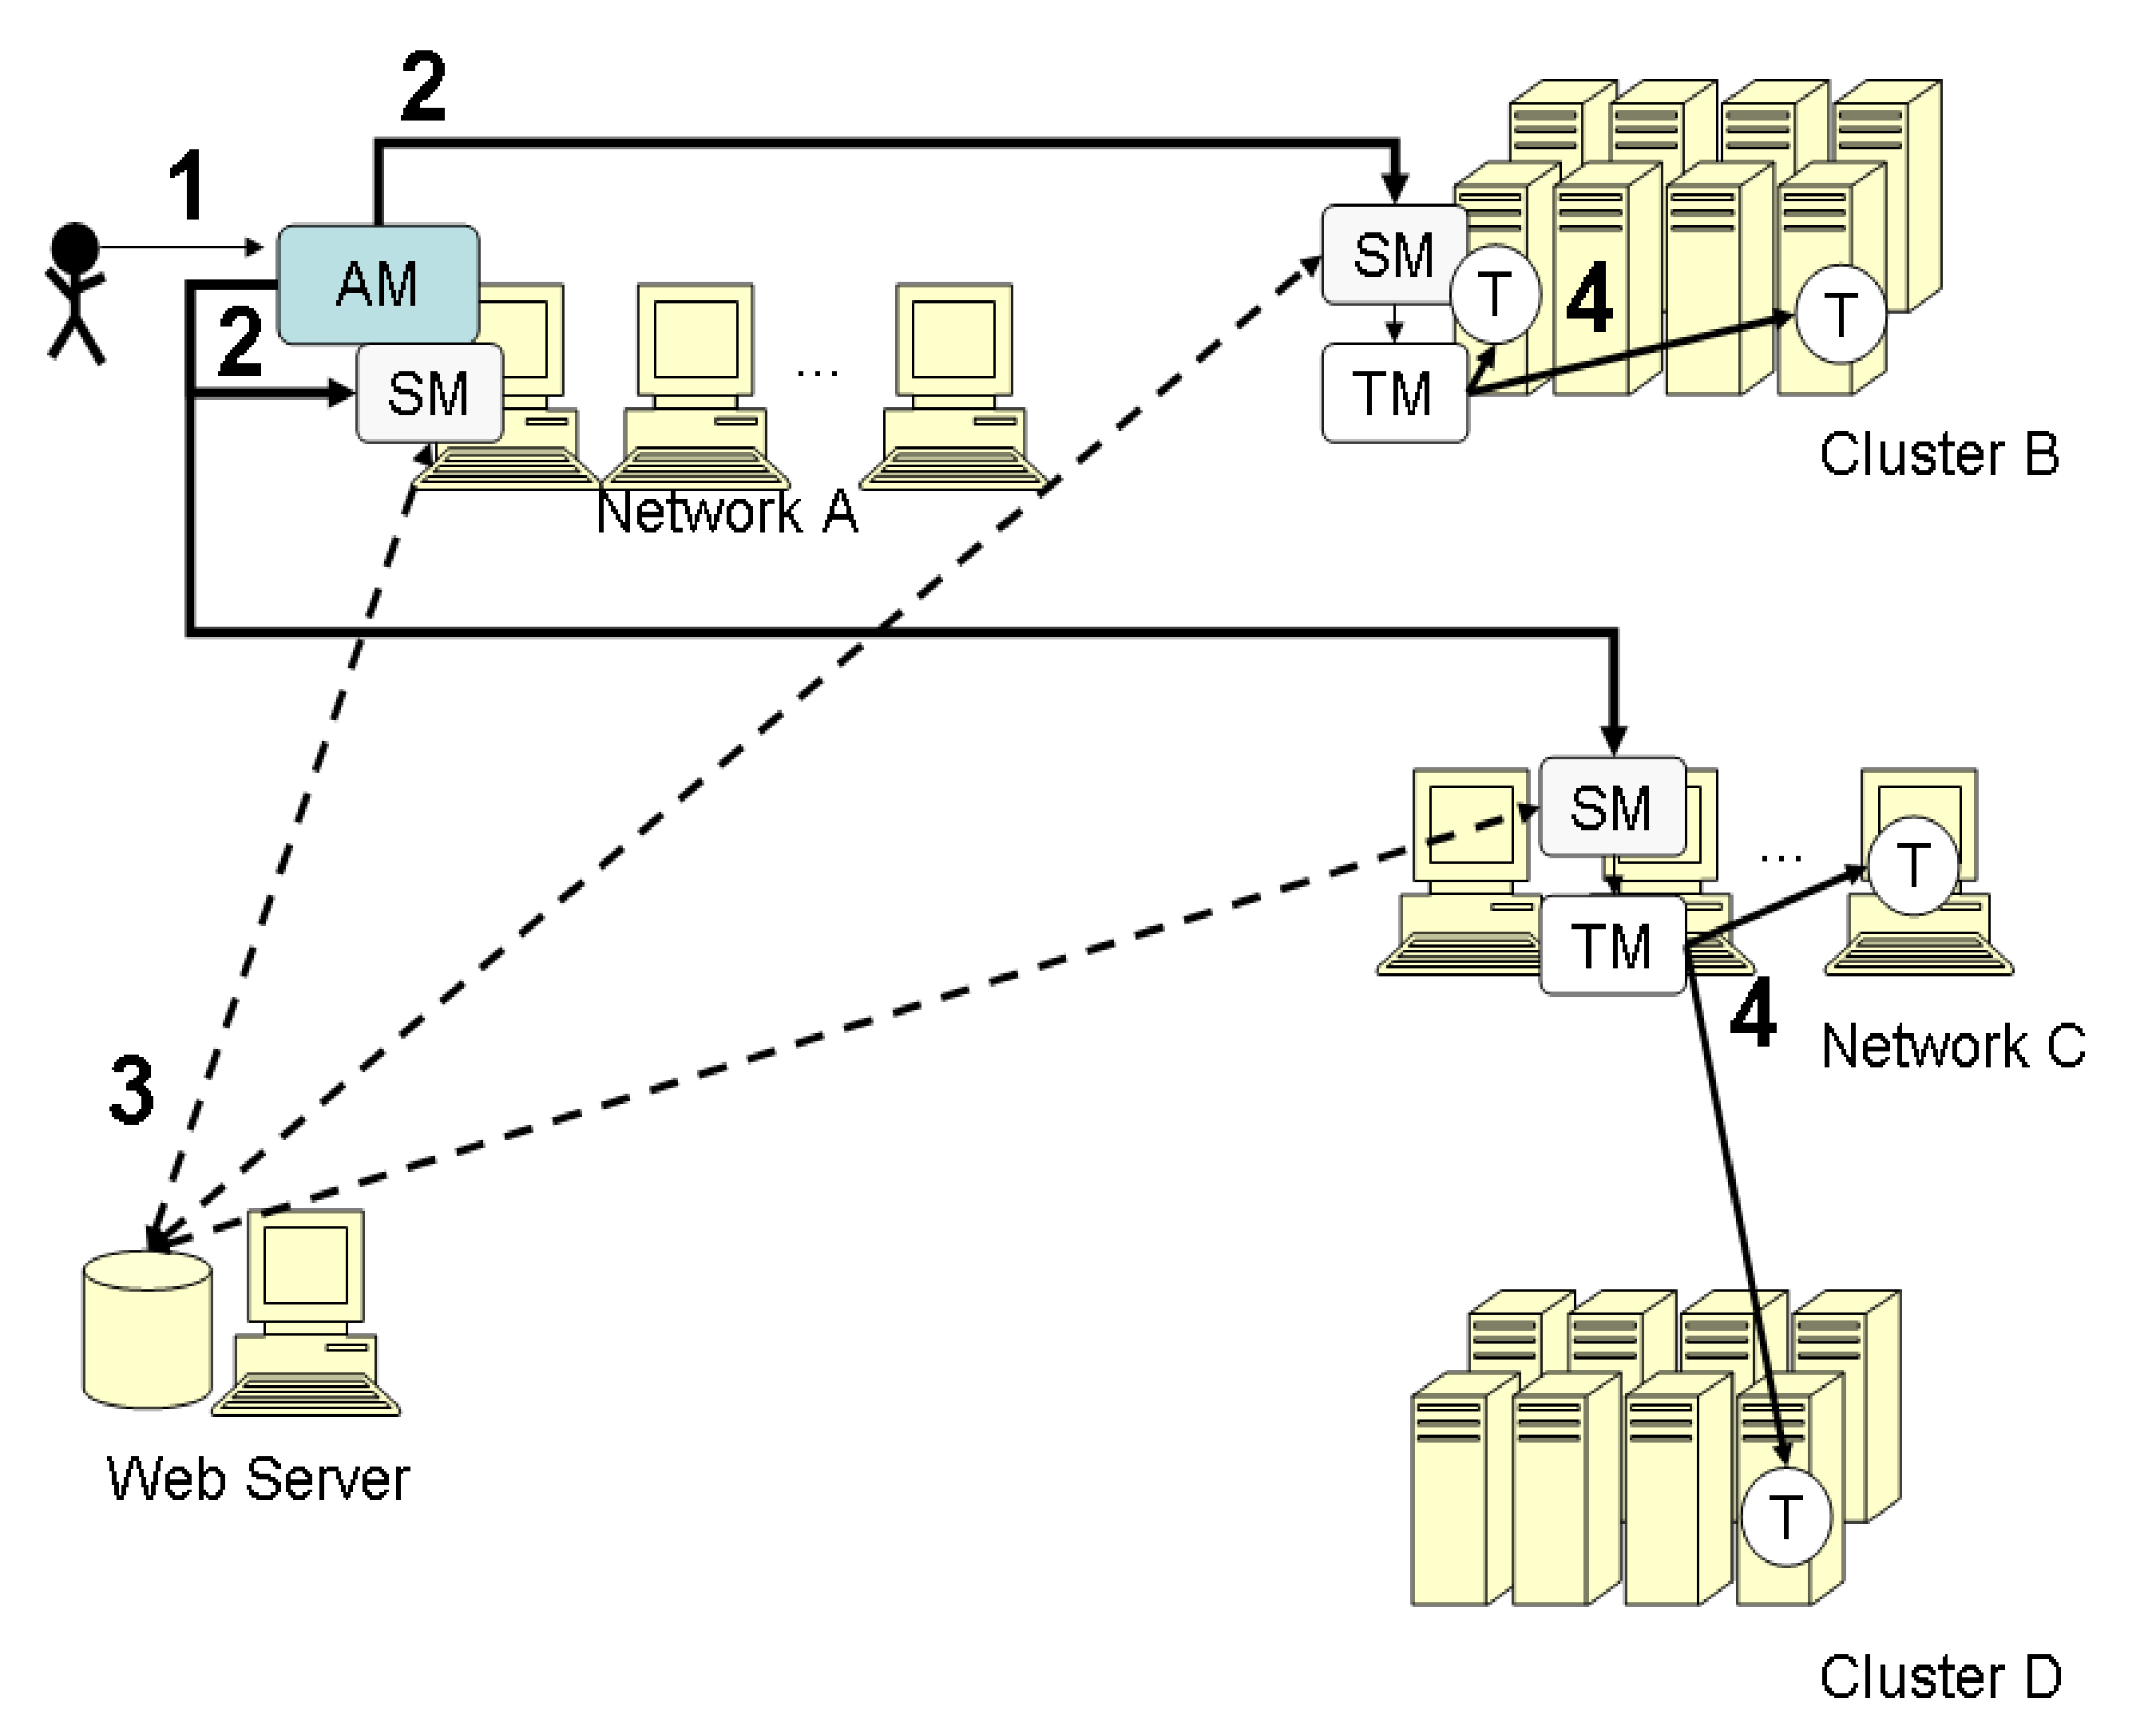
\includegraphics[scale=0.13]{./img/AppMan.eps}
\caption{AppMan executando principais passos}
\label{fig:AppMan}
\end{center}
\end{figure}

O capítulo seguinte demonstra as características da interface DRMAA usada na implementação do projeto junto com a Java \emph{Binding}.